% PGF style template to be used in the ktikz program
\documentclass[a4paper,twoside,11pt]{book}
\usepackage[dvipsnames]{xcolor}
\usepackage{amsmath}
\usepackage{relsize}
\usepackage{DejaVuSans}
\usepackage[T1]{fontenc}

\usepackage[charter]{mathdesign}
\DeclareFontFamily{OMS}{mdbch}{\skewchar\font=48}
\DeclareFontShape{OMS}{mdbch}{m}{n}{<->s*[0.96] mdbchr7y}{}
\DeclareFontShape{OMS}{mdbch}{m}{it}{<->ssub * mdbch/m/n}{}
\DeclareFontShape{OMS}{mdbch}{b}{n}{<->s*[0.96] mdbchb7y}{}
\DeclareFontShape{OMS}{mdbch}{bx}{n}{<->ssub * mdbch/b/n}{}
\usepackage{tikz}


\usetikzlibrary{arrows}
\usetikzlibrary{backgrounds}
\usetikzlibrary{calc}
\usetikzlibrary{fit}
\usetikzlibrary{positioning}
\usetikzlibrary{decorations}
\usetikzlibrary{decorations.shapes}
\usetikzlibrary{decorations.pathmorphing}
\usetikzlibrary{decorations.pathreplacing}
\usetikzlibrary{decorations.markings}
\usetikzlibrary{decorations.text}
\usetikzlibrary{matrix}
\usetikzlibrary{positioning}
\usetikzlibrary{shapes}
\usetikzlibrary{shapes.misc}
\usetikzlibrary{shapes.arrows}
\usetikzlibrary{shapes.multipart}
\usetikzlibrary{shadows}
\usetikzlibrary{spy}


\pgfdeclarelayer{background}
\pgfdeclarelayer{backbackground}
\pgfdeclarelayer{backbackbackground}
\pgfdeclarelayer{foreground}
\pgfsetlayers{backbackbackground,backbackground,background,main,foreground}
%\usepackage{color}
\usepackage[active,pdftex,tightpage]{preview}
\PreviewEnvironment[]{tikzpicture}
\PreviewEnvironment[]{pgfpicture}
\InputIfFileExists{../macros.tex}{}{
  \InputIfFileExists{macros.tex}{}%
}

\begin{document}
\def\mySecStr#1{\expandafter {\tt #1}\& }
\def\mySecStrAll#1{\ifx#1\mySecStrAll\else\mySecStr#1\expandafter\mySecStrAll\fi}
\def\mySeq#1{\expandafter {#1}\&}
\def\mySeqAll#1{\ifx#1\mySeqAll\else\mySeq#1\expandafter\mySeqAll\fi}


\newcommand{\YRNA}[6][]{
\begin{tikzpicture}[baseline={([yshift=-.5ex]rna)}]
  \matrix[matrix of nodes,nodes=cell,ampersand replacement=\&] (rna){
		\ifthenelse{\equal{#2}{}}{}{ \mySeqAll #2 \mySeqAll\\}
		};
\ifthenelse{\equal{#3}{}}{}{%
	\foreach \x/\y in {#3}{\draw (rna-1-\x) edge[ybp0] (rna-1-\y);}%
}
\ifthenelse{\equal{#4}{}}{}{%
	\foreach \x/\y in {#4}{\draw (rna-1-\x) edge[ybp1] (rna-1-\y);}%
}
\ifthenelse{\equal{#5}{}}{}{%
	\foreach \x/\y in {#5}{\draw (rna-1-\x) edge[ybp2] (rna-1-\y);}%
}
\ifthenelse{\equal{#6}{}}{}{%
	\foreach \x/\y in {#6}{\draw (rna-1-\x) edge[ybp3] (rna-1-\y);}%
}
\ifthenelse{\equal{#1}{}}{}{%
	\foreach \x/\y/\b/\a in {#1}{%
		\coordinate (X) at ($ (rna-1-\x)!.5!(rna-1-\y) $);%
		\draw ($ (X) - (0,\b) $) -- ($ (X) + (0,\a) $);%
	}%
}
\end{tikzpicture}}

\colorlet{blueprintcol}{gray!50!black}

\tikzstyle{ybp0}=[line width=1pt,draw=blue,in =90,out=90,looseness=1]
\tikzstyle{ybp1}=[line width=1pt,draw=red,in =-90,out=-90,looseness=1]
\tikzstyle{ybp2}=[line width=1pt,draw=green!60!black,in =-90,out=-90,looseness=1]
\tikzstyle{ybp3}=[line width=1.5pt,draw=red,in =90,out=90,looseness=1]
\tikzstyle{bp}=[line width=1pt,draw=blue,in =95,out=85,looseness=1.3]
\tikzstyle{altbp}=[line width=1pt,draw=red,dashed,in =95,out=85,looseness=.5]
\tikzstyle{cell}=[inner sep=0,minimum width=10pt,minimum height=11pt,font=\sf]


      \tikzstyle{baseedge}=[draw=gray!80, line width=1.2pt]

      
      \tikzstyle{cc1}=[draw=purple!50, line width=1.5pt]
      \tikzstyle{cc2}=[cc1,draw=green!70!black]
      \tikzstyle{cc3}=[cc1,draw=cyan!90!black]
      \tikzstyle{cc4}=[cc1,draw=gray]


      \tikzstyle{subcaption}=[font=\rm\relsize{+2}]
 
\begin{tikzpicture}

      \begin{scope}[shift={(2.4cm,11cm)}]
	    \node (input) {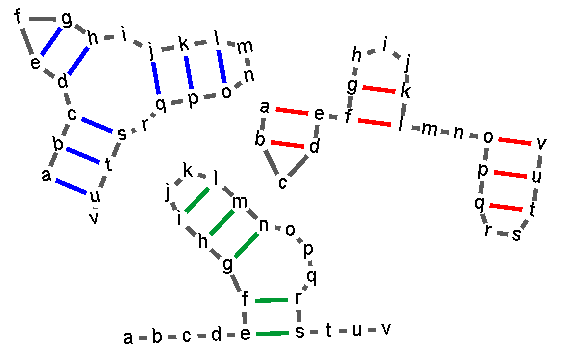
\includegraphics[scale=.8]{Bundled-Structs}};
        \node at (-2.25,1.25) {\relsize{+3}$R_1$};
        \node at (-.11,-1.2) {\relsize{+3}$R_2$};
        \node at (2.31,1.1) {\relsize{+3}$R_3$};
      \end{scope}
      \node[subcaption,below=5pt of input] (cap1) {i) Input Structures};

	  \node[right=55pt  of input] (merged)  {\YRNA{abcdefghijklmnopqrstuv}{1/21,2/20,3/19,4/8,5/7,10/17,11/16,12/15}%
    {1/5,2/4,6/12,7/11,15/22,16/21,17/20}{5/19,6/18,7/14,8/13,9/12}{}};
      \node[subcaption] at (merged |- cap1){ii) Merged Base-Pairs};

    
  
    \begin{scope}[xshift=19cm,yshift=9cm] 
      \node[cell] at (2,2) (node-1-1) {a};
      \node[cell] at (1,2) (node-1-5) {e};
      \node[cell] at (0,2) (node-1-7) {g};
      \node[cell] at (1,1) (node-1-16) {p};
      \node[cell] at (2,1) (node-1-21) {u};
      \node[cell] at (0,1) (node-1-11) {k};
      \node[cell] at (2,3) (node-1-3) {c};
      \node[cell] at (1,3) (node-1-19) {s};
      \node[cell] at (0,3) (node-1-14) {n};

      \node[cell] at (5,1)  (node-1-10) {j};
      \node[cell] at (5,2)  (node-1-17) {q};
      \node[cell] at (4,2) (node-1-20) {t};
      \node[cell] at (3,2) (node-1-2) {b};
      \node[cell] at (3,3)  (node-1-4) {d};
      \node[cell] at (4,3)  (node-1-8) {h};
      \node[cell] at (5,3) (node-1-13) {m};

      \node[cell] at (2,0) (node-1-6) {f};
      \node[cell] at (3,0) (node-1-12) {l};
      \node[cell] at (4,0) (node-1-15) {o};
      \node[cell] at (4,1) (node-1-22) {v};
      \node[cell] at (3,1) (node-1-9) {i};
      \node[cell] at (1,0) (node-1-18) {r};

      \draw (node-1-1) edge[baseedge] (node-1-21);
      \draw (node-1-5) edge[baseedge] (node-1-7);
      \draw (node-1-11) edge[baseedge] (node-1-16);
      \draw (node-1-1) edge[baseedge] (node-1-5);
      \draw (node-1-21) edge[baseedge] (node-1-16);
      \draw (node-1-7) edge[baseedge] (node-1-11);
      \draw (node-1-4) edge[baseedge] (node-1-8);
      \draw (node-1-4) edge[baseedge] (node-1-2);
      \draw (node-1-2) edge[baseedge] (node-1-20);
      \draw (node-1-20) edge[baseedge] (node-1-17);
      \draw (node-1-17) edge[baseedge] (node-1-10);
      \draw (node-1-6) edge[baseedge] (node-1-12);
      \draw (node-1-12) edge[baseedge] (node-1-15);
      \draw (node-1-15) edge[baseedge] (node-1-22);
      \draw (node-1-3) edge[baseedge] (node-1-19);

      \draw (node-1-5) edge[baseedge] (node-1-19);
      \draw (node-1-6) edge[baseedge] (node-1-18);
      \draw (node-1-7) edge[baseedge] (node-1-14);
      \draw (node-1-8) edge[baseedge] (node-1-13);
      \draw (node-1-9) edge[baseedge] (node-1-12);

 
	  \tikzstyle{cc1}+=[line width=2.5pt]
      
      \draw (node-1-1) edge[cc1] (node-1-21);
      \draw (node-1-5) edge[cc1] (node-1-7);
      \draw (node-1-11) edge[cc1] (node-1-16);
      \draw (node-1-1) edge[cc1] (node-1-5);
      \draw (node-1-21) edge[cc1] (node-1-16);
      \draw (node-1-7) edge[cc1] (node-1-11);
      \draw (node-1-7) edge[cc1] (node-1-14);
      \draw (node-1-5) edge[cc1] (node-1-19);
      \draw (node-1-3) edge[cc1] (node-1-19);



      \draw (node-1-4) edge[cc4] (node-1-8);
      \draw (node-1-4) edge[cc4] (node-1-2);
      \draw (node-1-2) edge[cc4] (node-1-20);
      \draw (node-1-20) edge[cc4] (node-1-17);
      \draw (node-1-17) edge[cc4] (node-1-10);
      \draw (node-1-8) edge[cc4] (node-1-13);

      \draw (node-1-6) edge[cc3] (node-1-12);
      \draw (node-1-12) edge[cc3] (node-1-15);
      \draw (node-1-15) edge[cc3] (node-1-22);
      \draw (node-1-6) edge[cc3] (node-1-18);
      \draw (node-1-9) edge[cc3] (node-1-12);
      \node (midpoint) at (2.5,0) {};
    \end{scope}
      \node[subcaption] at (midpoint|-cap1) {iii) Compatibility Graph};

      \begin{scope}[yshift=+14.5em, 
  sibling distance = 4em,
  level distance = 2em,
  every node/.style = {tdnodes}]]
  \tikzstyle{tdnodes}=[shape=rectangle, font=\sf,
    draw, align=center]
  \node at (2,1) (root) {$\varnothing$};
 
  \tikzstyle{tdnodes}=[shape=rectangle, font=\sf,
    draw, align=center,draw=cyan!90!black,line width=1.5pt]

  \node (r1) {v o} 
      child 
      { 
        node {o l} 
        child 
        { 
          node {l f} 
          child 
          { 
            node {f r} 
          }
        }
        child 
        { 
          node {l i} 
        }
      }
;
  \tikzstyle{tdnodes}+=[draw=gray,line width=1.5pt]

  \node (r2) at (2,0) {j q} 
      child 
      { 
        node {q t} 
        child  
        { 
          node {t b} 
          child 
          { 
            node {b d} 
          child 
          { 
            node {d h} 
          child 
          { 
            node {h m} 
          }
          }
          }
        }
      };

  \tikzstyle{tdnodes}+=[draw=purple!50,line width=1.5pt]

  \node (r3) at (4,0) {k p} 
      child 
      { 
        node {k p g} 
        child 
        { 
          node {g n} 
        }
        child 
        { 
          node {g p u} 
          child 
          { 
            node {u g e} 
            child 
            { 
              node {u e a} 
            }
            child 
            { 
              node {e s} 
              child 
              { 
                node {s c} 
              }
            }
          }
        }
      };
   \draw (root) edge (r1);
   \draw (root) edge (r2);
   \draw (root) edge (r3);

   \node[subcaption, below=4cm of r2, draw=none] (lbl2) {iv) Tree Decomposition};

	 \end{scope} 

        \tikzstyle{nts} = [inner sep=0,font=\sf\relsize{-2}, anchor=south]
      \begin{scope}[yshift=+14em,xshift=5cm]
       \node[] (sarr) {}; 
       \node[right=4.9cm of sarr] (farr) {}; 
       \draw (sarr) edge[-triangle 45,line width=3pt,blueprintcol] node[above=5pt,inner sep=0, pos=.48] (abovetxt) {\texttt{RNARedPrint}} node[below=5pt, text width =7.5em,draw=none,text centered,font=\relsize{-1},fill=none,inner sep=0, pos=.48]  (belowtxt) {Partition Function\\ Stochastic Backtrack} (farr);
       \node[fit= (abovetxt)  (belowtxt),draw,line width=2pt,inner sep=3pt,rounded corners=5pt,blueprintcol] (redprint) {}; 
     \node[rounded corners=10pt, draw=blueprintcol,fill=blueprintcol!2!white,line width=2pt] (distribs) at (9.2,-1.) {\scalebox{.8}{\begin{tikzpicture}\newcommand{\Angle}{15}
	   \node[rotate=\Angle,nts] at (6,0){GACUUUAGCUUGUUUGAAGUUA};
	   \node[rotate=\Angle,nts] at (6,-.35){GACUUGGGACUUUUAGGUGUCU};
	   \node[rotate=\Angle,nts] at (6,-.7){UUAGAUUCCAGGGGCUUGUAGG};
	   \node[rotate=\Angle,nts] at (6,-1.05){GGUUUAGGGCCUUUAGGUAUCU};
	   \node[rotate=\Angle,nts] at (6,-1.4){AUUGUGACGGUCGUGACUAGUU}; 
	   \node[rotate=\Angle,nts] at (6,-1.75){\relsize{+2}$\ldots$}; 
      \begin{scope}[shift={(8.4cm,-1.7cm)}]
	   \node at (0,0){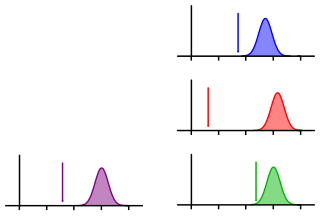
\includegraphics{distribTemp}}; 
       \node at (4,1.1) {\relsize{-1}$0$};
       \node at (4,-1.0) {\relsize{-1}$0$};
       \node at (4,-3.1) {\relsize{-1}$0$};

       \node at (3.2,1.1) {\relsize{-1}$-5$};
       \node at (3.2,-1.0) {\relsize{-1}$-5$};
       \node at (3.2,-3.1) {\relsize{-1}$-5$};

       \node at (1.5,1.1) {\relsize{-1}kcal.mol$^{-1}$};
       \node at (1.5,-1.0) {\relsize{-1}kcal.mol$^{-1}$};
       \node at (1.5,-3.1) {\relsize{-1}kcal.mol$^{-1}$};
  
       \node (tmp) at (.4,2.25) {\relsize{+2}$E_1$};
       \node[below=1.42cm of tmp] (tmp) {\relsize{+2}$E_2$};
       \node[below=1.42cm of tmp] (tmp) {\relsize{+2}$E_3$};

       \node at (-4.7,-2.05)  {\relsize{+2}{\sf GC}\%};
       \node at (-3.95,-3.1) {\relsize{-1}$0$};
       \node at (-2.43,-3.1) {\relsize{-1}$50$};
       \node at (-0.89,-3.1) {\relsize{-1}$100$};
	 \end{scope}
\end{tikzpicture}}
};    
        \node[subcaption,xshift=-3em] at (distribs|-lbl2) {v) Weight Optimization (Adaptive Sampling)};

     \node at ($(distribs.south west)+(0,.5)$) (tmp) {};
	 \draw[line width=3pt,rounded corners=40pt,-triangle 45,blueprintcol,postaction={decoration={text along path,
  text = {Weights update}, text align=fit to path, text color = blueprintcol,
  pre length=1.6em, post length=2.5em,raise=.8em},decorate}] (tmp.center)  -|  (redprint);

	 \end{scope}


	 \begin{scope}

     \node[rounded corners=10pt, ] (distribsfinal) at (21.8,4) {\scalebox{.9}{\begin{tikzpicture}\newcommand{\Angle}{15}
      \begin{scope}[shift={(8.4cm,-1.7cm)}]
		\newcommand{\Shift}{4pt}
	   \node[nts] (tmp) at (-2.7,2.5)         {GCCGCGGUAGCUACAGCCGGCU};
	   \node[nts,below=\Shift of tmp] (tmp) {UUGGGGUUGGGUAGACUCCGGU};
   	   \node[nts,below=\Shift of tmp] (tmp) {GCUGCAGCGGCUGUGGCUGGCC};
	   \node[nts,below=\Shift of tmp] (tmp) {GGUUCUGGUUUGCUUAGGGCUA};
   	   \node[nts,below=\Shift of tmp] (tmp) {CGACGGCGGUGCCGGCAUUUGC};
	   \node[nts,below=\Shift of tmp] (tmp) {\relsize{+2}\ldots};


	   \node at (-2.4,-1.25){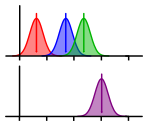
\includegraphics{distribFinal}}; 
       \node at (-0.85,-1.35) {\relsize{-1}$0$};
       \node at (-2.89,-1.35) {\relsize{-1}kcal.mol$^{-1}$};

       \node (tmp) at (-4.7,-.25) {\relsize{+1}$E_1$};
       \node[below=-7pt of tmp] (tmp) {\relsize{+1}$E_2$};
       \node[below=-7pt of tmp] (tmp) {\relsize{+1}$E_3$};

       \node at (-4.7,-2.05)  {\relsize{+2}{\sf GC}\%};
       \node at (-3.95,-3.1) {\relsize{-1}$0$};
       \node at (-2.43,-3.1) {\relsize{-1}$50$};
       \node at (-0.89,-3.1) {\relsize{-1}$100$};
	 \end{scope}
\end{tikzpicture}}
};    

      \node[subcaption, text width=14em,text centered ] at (lbl2-|distribsfinal) {vi) Final Designs};

	 \end{scope}



\end{tikzpicture}
\end{document}
